%%%%%%%%%%%%%%%%%%%%%%%%%%%%%%%%%%%%%%%%%
% Thin Sectioned Essay
% LaTeX Template
% Version 1.0 (3/8/13)
%
% This template has been downloaded from:
% http://www.LaTeXTemplates.com
%
% Original Author:
% Nicolas Diaz (nsdiaz@uc.cl) with extensive modifications by:
% Vel (vel@latextemplates.com)
%
% License:
% CC BY-NC-SA 3.0 (http://creativecommons.org/licenses/by-nc-sa/3.0/)
%
%%%%%%%%%%%%%%%%%%%%%%%%%%%%%%%%%%%%%%%%%

%----------------------------------------------------------------------------------------
%	PACKAGES AND OTHER DOCUMENT CONFIGURATIONS
%----------------------------------------------------------------------------------------

\documentclass[a4paper, 11pt]{article} % Font size (can be 10pt, 11pt or 12pt) and paper size (remove a4paper for US letter paper)
\usepackage{color}
\usepackage[protrusion=true,expansion=true]{microtype} % Better typography
\usepackage{graphicx} % Required for including pictures
\usepackage{wrapfig} % Allows in-line images
\usepackage{endnotes}
\usepackage{mathpazo} % Use the Palatino font
\usepackage[T1]{fontenc} % Required for accented characters
\linespread{1.05} % Change line spacing here, Palatino benefits from a slight increase by default
\usepackage{fancyhdr}
\usepackage[margin=1.25in]{geometry}
\pagestyle{fancy}
\fancyhf{}
\rhead{Machine Learning Problem Set 4, 14.03.2019}
\lhead{Felix Adam}
\rfoot{Page \thepage}
\usepackage{amsmath}
\usepackage{amssymb}
\usepackage{version}
\usepackage{setspace}
\usepackage{enumerate}
\usepackage{multicol}
\usepackage{amsfonts}
\usepackage{amssymb}
\usepackage{graphicx}
\usepackage{rotating}
\usepackage{lscape}
\usepackage{pdflscape}
\usepackage{array,tabularx,float,dcolumn,lscape}
\usepackage{booktabs}
\usepackage{xr}
\usepackage{dcolumn}
\usepackage{hyperref} 
\usepackage{amsmath}
\usepackage{algorithm}
\usepackage[noend]{algpseudocode}
\graphicspath{ {../01_Figures/} }

\makeatletter
\def\BState{\State\hskip-\ALG@thistlm}
\makeatother

\newlength\tindent
\setlength{\tindent}{\parindent}
\setlength{\parindent}{0pt}
\renewcommand{\indent}{\hspace*{\tindent}}
\renewcommand{\familydefault}{\sfdefault}

\makeatletter
\renewcommand\@biblabel[1]{\textbf{#1.}} % Change the square brackets for each bibliography item from '[1]' to '1.'
\renewcommand{\@listI}{\itemsep=0pt} % Reduce the space between items in the itemize and enumerate environments and the bibliography

\renewcommand{\maketitle}{ % Customize the title - do not edit title and author name here, see the TITLE block below
\begin{flushright} % Right align
{\LARGE\@title} % Increase the font size of the title

\vspace{50pt} % Some vertical space between the title and author name

{\large\@author} % Author name
\\\@date % Date

\vspace{40pt} % Some vertical space between the author block and abstract
\end{flushright}
}

\begin{document}

\section*{Problem 12} 

We have the cost functional $A(f)=E[\phi(-f(x) y)$ and need to determine the function $f^*$ that minimizes $A(f)$. 

First, we apply the law of iterated expectations, taking expectations with respect to $x$.

$$E[\phi(-f(x) y)]=E[E[\phi(-f(x) y) | x]]$$

Minimizing this is equivalent to minimizing the inner expectations with respect to $x$. 

$$E[\phi(-f(x) y) | x] = \eta(x) \cdot \phi(-f(x))+(1-\eta(x)) \phi(f(x))  $$

where $\eta(x) = P(Y = 1 | x)$

Now optimizing with respect to $f$ yields the following first order condition:

$$-\eta(x) \cdot \phi^{\prime}(-f(x))+(1-\eta(x)) \phi^{\prime}(f(x))=0$$

We get that the optimal function $f^*$ satisfies the following ratio:

$$\frac{\phi^{\prime}(f^*(x))}{\phi^{\prime}(-f^*(x))}=\frac{\eta(x)}{1-\eta(x)}$$

Defining $\frac{\phi^{\prime}(f(x))}{\phi^{\prime}(-f(x))} = \theta(f(x))$ we get that the optimal f satisfies

$$f^* = \theta^{-1}\left(\frac{\eta(x)}{1-\eta(x)} \right)$$
\\
Now we need to show that the classifier $g(x) = sgn(f^*(x))$ is the Bayes classifier. From the previous result we have that if $\eta(x) > (1-\eta(x))$ then $\phi^{\prime}(f(x)) > \phi^{\prime}(-f(x))$. 

We know that $\phi^{\prime}$ is a positive function. Therefore if  $\phi^{\prime}(f(x)) > \phi^{\prime}(-f(x))$ we have that $f^*(x) >0 $, consequently $sign( f^*(x) ) \leftrightarrow  \eta(x) > \frac{1}{2}$. Which is the Bayes classifier.

\section*{Problem 13}

We have the feature mapping $(\Phi(x))_{n}=\frac{1}{\sqrt{n !}} x^{n} e^{-\frac{x^{2}}{2}}$. We can determine the kernel function in the following way:

\begin{align*}
K(x,y) &= \langle\Phi(x), \Phi(y)\rangle =  \sum_{n=0}^{\infty} \phi (x)_n \phi (y)_n \\
&= \sum_{n=0}^\infty \frac{1}{\sqrt{n !}} x^{n} e^{-\frac{x^{2}}{2}} \cdot \frac{1}{\sqrt{n !}} y^{n} e^{-\frac{y^{2}}{2}} \\
&= \sum_{n=0}^\infty \frac{1}{n !}(y  x)^{n} e^{-\frac{x^{2}+y^2}{2}}  \\ 
&= e^{xy} \cdot e^{-\frac{x^2 + y^2}{2}} \\
&= e^{-\frac{1}{2} \left( x^2 + y^2 - 2xy \right)} \\
&= e^{-\frac{1}{2} (x-y)^2}
\end{align*}

We can generalize this for $\mathbb{R}^{d} \times \mathbb{R}^{d}$

\begin{align*}
K(x,y) &= \sum_{n=0}^{\infty} \frac{1}{n !}\left(x^{T} y\right)^{n} e^{-\frac{x^{T} 
x +  y^{T} y }{2}}  \\
&= e^{x^T y} \cdot e^{- \frac{x^Tx + y^Ty}{2}} \\
&= e^{- \frac{1}{2} (x^Tx + y^Ty - 2xy^T} \\
&= e^{-\frac{1}{1} (x-y)^T(x-y)}
\end{align*}

The corresponding feature mapping is:

\begin{align*}
\phi(x)_n = \frac{1}{\sqrt{n !}} x^{n} \cdot e^{-\frac{x^{T}x}{2}} 
&= \frac{1}{\sqrt{n !}} x^{n} \cdot e^{-\frac{\|x\|^{2}}{2}}
\end{align*}

\section*{Problem 14}

Define $f_w(*)  = K(*,w)$ and the Rademacher average $\mathbf{E} \sup _{w \in \mathcal{X}} \frac{1}{n} \sum_{i=1}^{n} \sigma_{i} f_{w}\left(x_{i}\right)$

\begin{align*}
R(f_w) &= E  \sup_{w \in \chi} \frac{1}{n} \sum_{i=1}^n \sigma_i f_w(x_i) \\
&= E \sup_{w \in \chi} \frac{1}{n} \sum_{i=1}^n \sigma_i K(x_i,w)\\
&= E \sup_{w \in \chi} \frac{1}{n} \sum_{i=1}^n \sigma_i \langle w, x_i\rangle \\
&= E \sup_{w \in \chi} \frac{1}{n} \langle w, \sum_{i=1}^n \sigma_i x_i \rangle \\
&= E \sup \frac{1}{n} \langle w \frac{\sum_{i=1}^n \sigma_i x_i}{\| \sum_{i=1}^n \sigma_i x_i \| },  \sum_{i=1}^n \sigma_i x_i \rangle
\end{align*}

Now we can use that $\sup w^T a = \| a \|$ for $||w|| \leq 1$, so for $\| w \| \leq 1$:

\begin{align*}
R(f_w) &= E \frac{1}{n} \langle  \frac{\sum_{i=1}^n \sigma_i x_i}{\| \sum_{i=1}^n \sigma_i x_i \| },  \sum_{i=1}^n \sigma_i x_i \rangle \\
&= E \frac{1}{n} \langle  \sum_{i=1}^n \sigma_i x_i ,  \sum_{i=1}^n \sigma_i x_i  \rangle \\
&= E\frac{1}{n}\left\|\sum_{i=1}^{n} \sigma_{i} x_{i}\right\| \\
&= E\frac{1}{n} \sqrt{\left\|\sum_{i=1}^{n} \sigma_{i} x_{i}\right\|^2 }
\end{align*}

Now, applying Jensens inequality 

\begin{align*}
R(f_w) & \leq \frac{1}{n} \sqrt{ E \left\|\sum_{i=1}^{n} \sigma_{i} x_{i}\right\|^2 } \\
&= \frac{1}{n} \sqrt{ E \left[ \sum_{i=j} \left\| x_i \sigma_i \right\|^2 \right] + 2 E \left[ \sum_{i<j} \left\| x_i \sigma_i \sigma_j x_j \right\|^2 \right]} \\
&= \frac{1}{n} \sqrt{E \left[ \sum_{i=j} \left\| \sigma_i x_i \right\|^2 \right]} \\
& = \frac{\sqrt{n}}{n} \sqrt{E \left[\left\| \sigma_i x_i \right\|^2 \right]} \\
& \leq \frac{1}{\sqrt{n}} * R = \frac{1}{\sqrt{n}}
\end{align*}

where $R=1$ since $k \in [-1,1]$

\section*{Problem 15}
To get a feel for the problem and the different classifiers, we can plot the data and the classifiers resulting from optimizing the different cost functions in $R^2$.

\begin{figure}[H] 
\centering
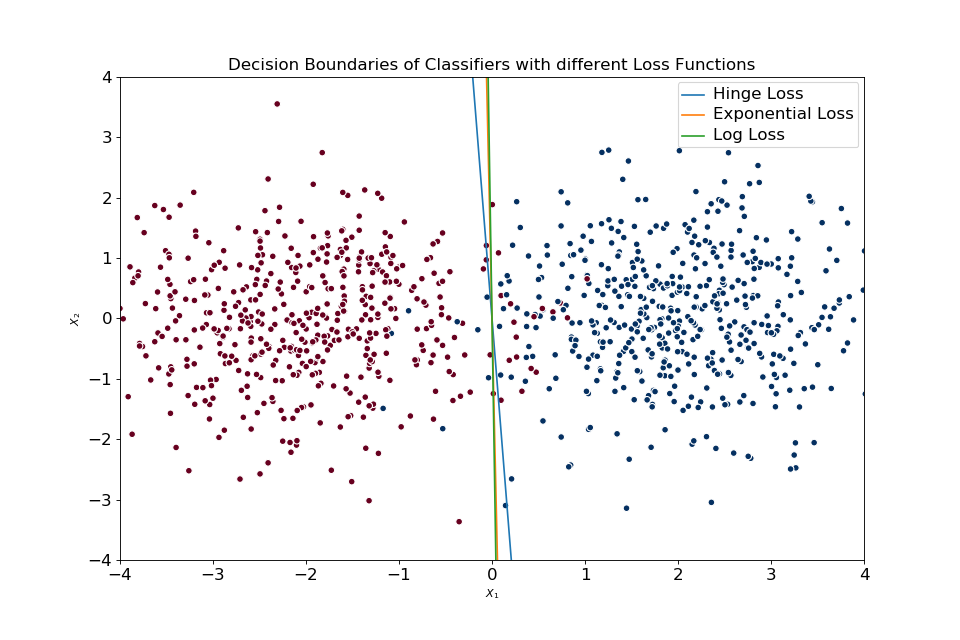
\includegraphics[scale=0.4]{Decisions_Boundaries}
\end{figure}

As in the previous problemset, we can see that the data is not linearly seperable, but it will be easier the larger the margin $a$ is. Further, in $R^2$ the resulting decision boundaries don't differ much. Differences could potentially arise from choosing different random data points when optimizing using stochastic gradient descent. 

\subsection*{Simulation Results}
\begin{figure}[H]
\centering
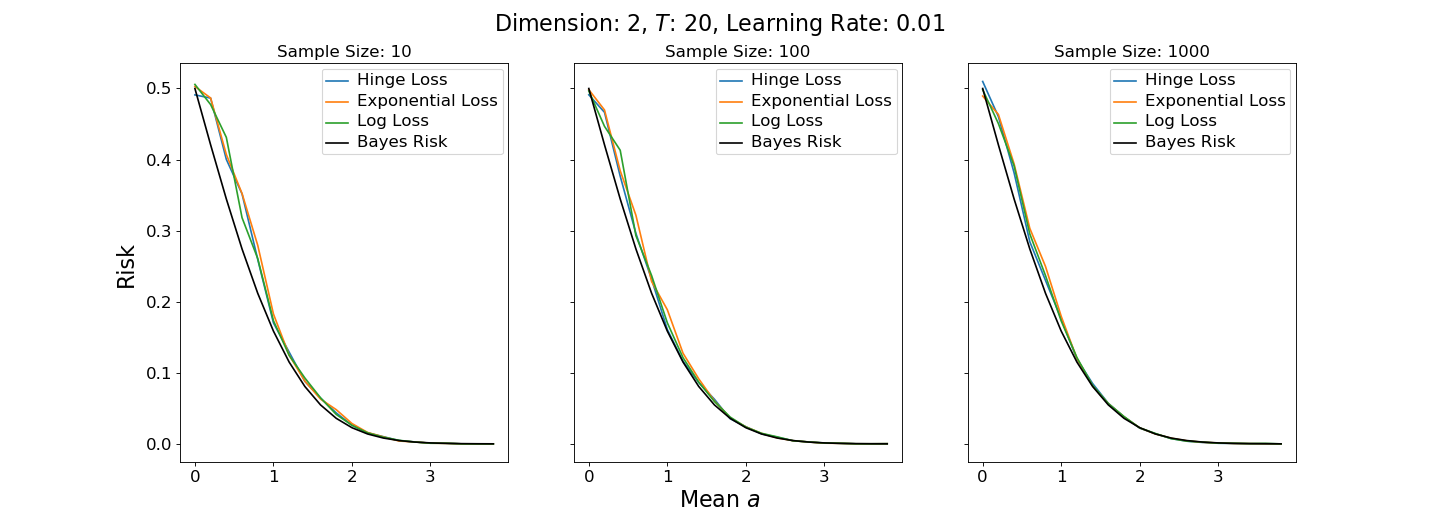
\includegraphics[scale=0.35]{Risk_Dimension_2}
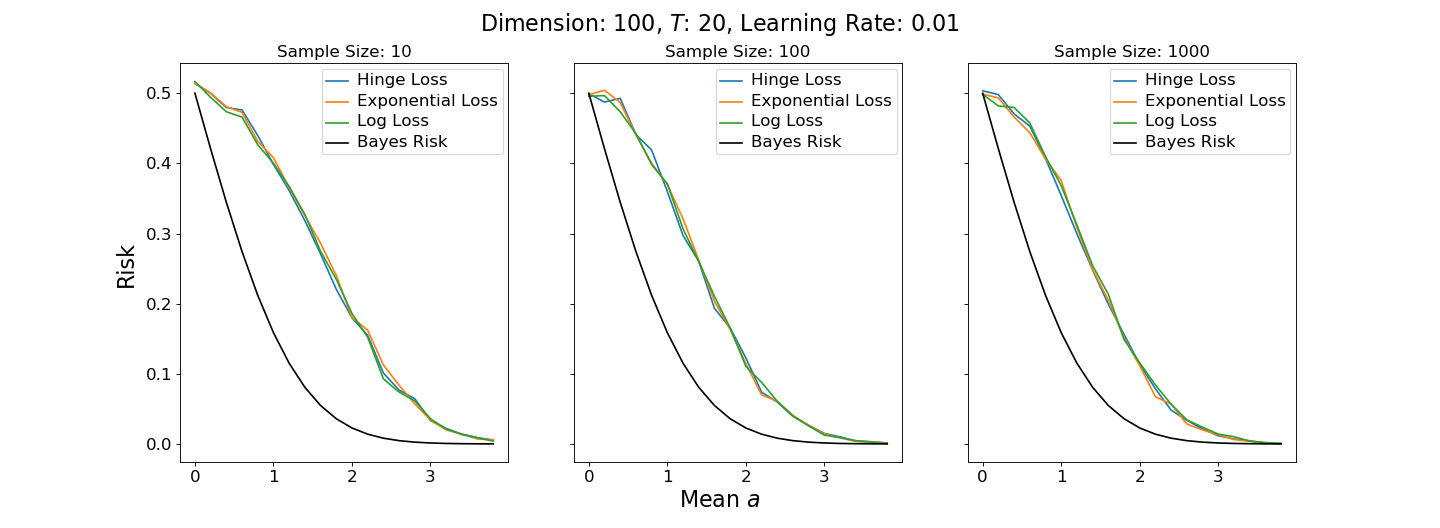
\includegraphics[scale=0.35]{Risk_Dimension_100}
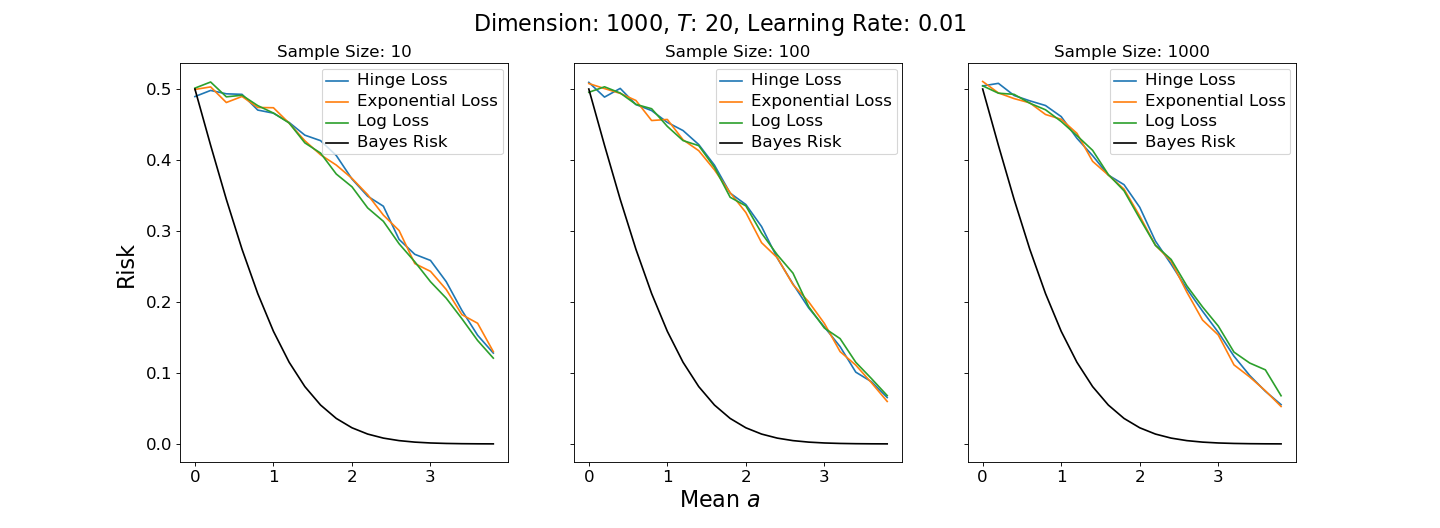
\includegraphics[scale=0.35]{Risk_Dimension_1000}
\end{figure}

The above simulations show the estimated risk of each classifier resulting from optimizing the various loss functions on the training data for corresponding sample size. At every step, the number of data points evaluated by the algorithm is only 20, with a learning rate of 0.01. First of all, we can see how exceptionally well stochastic gradient descent works! We only evaluate the loss function at 20 random points but still see that all classifiers converge towards the Bayes risk. \\
As expected, lower values of the margin $a$ result in higher overall risk for all classifiers. With larger margins, all classifiers converge to the Bayes risk. Further, there seems to be no difference between the risk of classifiers based on the different loss functions. As in the previous problem set, the overall risk of the classifiers increases with the number of dimensions, since each additional dimension just adds noise to the classification task.  Larger sample sizes seem to help with this problem, since all classifiers converge faster to the Bayes risk at a given margin $a$ with larger sample sizes.

\subsection*{Varying Learning Rate $\eta$ and Epochs $T$}

\begin{figure}[H]
\centering
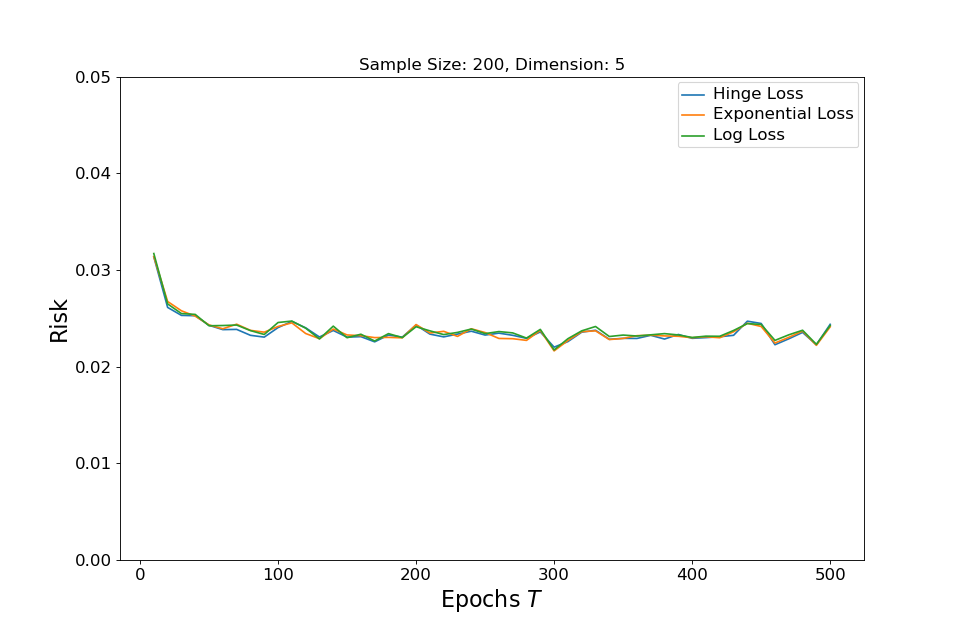
\includegraphics[scale=0.4]{Epochs}
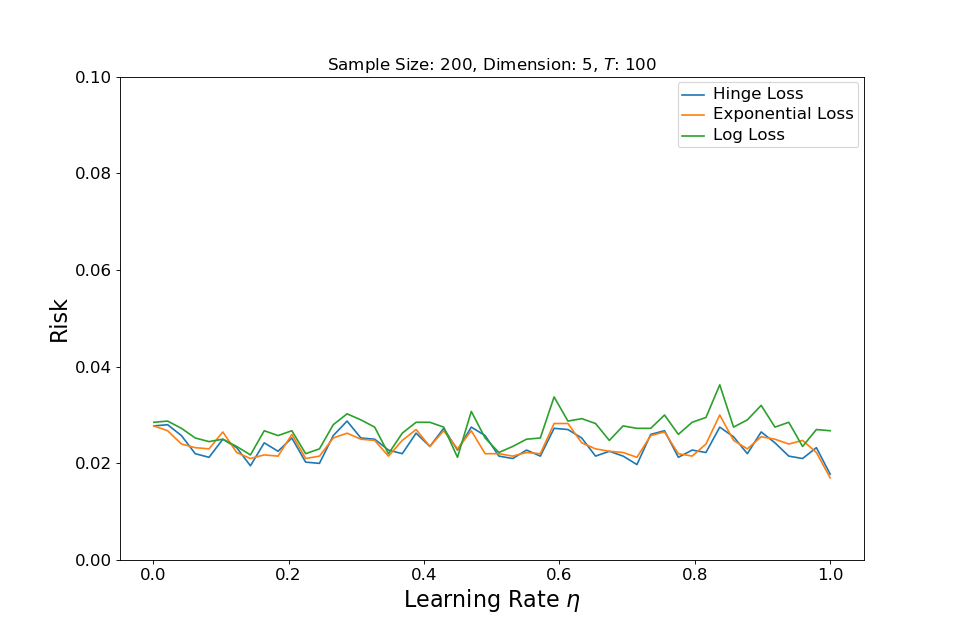
\includegraphics[scale=0.4]{LearningRate}
\end{figure}

Note, that these plots arise from data with a margin $a=2$. 
Varying the number of data points $T$ which are evaluated by the aglorithm doesn't lead to a great improvment once $T$ exceeds 100. This could be due to the data not being linearly seperable at margin $a=2$, so more iterations can't lead to a better seperation. Similarly, varying the learning rate $\eta$ doesn't seem to improve performance, but rather it could actually lead to worse outcomes (in particular for the log-loss). In general one can note that the optimal number of iterations $T$ and the learning rate $\eta$ depend on factors like the margin, sample size, value of the gradient and others. As noted in class, one could use algorithms like Nesterovs Momentum to automatically deal with the learning rate. 

\end{document}


 